\chapter{Ergebnisse}
%Sandra
\Autor{Sandra Schröder}\\\\
Verfahren zur Skelettierung von Bildobjekten fordern bestimmte Eigenschaften an das Skelett \textbf{todo Quelle}. Dies ist zum einen die \emph{Konnektivität} des Skeletts. Dies bedeutet, dass es keine Lücken und Unterbrechungen im Skelett gibt. Ein zusammenhängendes Objekt sollte nämlich ein zusammenhängendes Skelett besitzen. 
Viele Skelettierungsverfahren fordern, dass ein Skelett genau 1 Pixel breit ist und \emph{zentriert} im ursprünglichen Objekt liegt. Zentiert bedeutet, dass der Abstand des Skeletts zum ursprünglichen Rand zu allen Seiten gleich groß ist.\\
Das das Skelett als Deskriptor für die Form eines Objektes dient, sollte es die geometrischen Eigenschaften und die Topologie des Objektes gut wiedergeben können.\\
Bilder sind immer mit Rauschen behaftet. Eine Skelettierung sollte, unabhängig davon, wie stark das Rauschen ausgeprägt ist, robust gegenüber solchen Störungen sein.\\
In den folgenden Abschnitten werden unsere Ergebnisse für die beiden Skelettierungsalgorithmen, die im
Rahmen dieser Projektarbeit entwickelt wurden, vorgestellt. Zur Bewertung der Ergebnisse greifen wir auf die
gewünschten Eigenschaften eines Skeletts zurück und überprüfen, ob die Algorithmen sie erfüllen.
\section{Vergleich der Algorithmen}
\subsection{Thinning}
\subsection{Distanztransformation}
Screenshots und Laufzeitmessungen
%Mittwoch
\newpage
\section{Verbesserung der Skelettqualität}
Das Skelett, welches mit der Methode der Distanztransformation bestimmt wurde, weist Lücken zwischen den Skelettteilen auf. Um die Topologie und geometrische Eigenschaften des Objekts gut wiederzugeben, ist ein lückenloses Skelett wünschenswert. \\
Die Ursache der Lücken sind der Gradientenbetrag, der für die Extraktion der Skelettlinie berechnet wurde und die Segmentierung des Gradientenbildes. Abbildung \ref{fig:hand-skelett} zeigt ein Beispiel dazu. Abbildung (a) ist das Originalbild mit dem Objekt, von dem das Skelett, wie in Abbildung (c) zu sehen, bestimmt wurde. Da der Algorithmus auf der Grundlage von Bildern arbeitet, bei denen das Objekt und der Hintergrund schwarz markiert sind,
wurde das Bild zuvor invertiert. Abbildung (b) zeigt die Distance Map des Originalbildes. Abbildung (d) ist das Gradientenbild der Distance Map. Das Gradientenbild wurde mit einem empirisch gewählten Schwellwert segmentiert, um anschließend die Skelettlinie zu extrahieren. Dadurch werden Linien im Gradientenbild, die einen kleineren Grauwert als der Schwellwert besitzen, eliminiert. 
\begin{figure}[htbp]
\centering
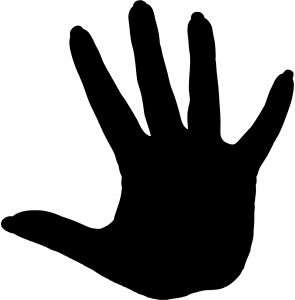
\includegraphics[width=1.0\linewidth]{./fig/hand}
\caption{Bestimmung des Skelett mittels Distanztransformation. (a) Originalbild (b) Distance Map (c) Gradientenbild (d) Skelett}
\label{fig:hand-skelett}
\end{figure}
In den folgenden Abschnitten werden Methoden zur Verbesserung des Skeletts vorgestellt. Dies umfasst zum einen die Herstellung Pixelkonnektivität beziehungsweise dem Füllen der Lücken zwischen den Skelettlinien. Zum anderen ist es wünschenswert, dass die Skelettlinie des Objektes nicht breiter als ein Pixel ist. Zuerst wurden markante Punkte auf dem Skelett bestimmt. Diese wurden
genutzt, um mittels Breitensuche und Tiefensuche Pfade zwischen ihnen zu finden und sie zu verbinden. Punkte werden miteinander
verbunden, wenn sie nah genug beieinander sind. Das Ergebnis ist ein Skelett
zusammenhängenden Skelettlinien. Die genaue Umsetzung der Algorithmen wird in den Abschnitten \ref{subsec:breitesuche} und \ref{subsec:tiefensuche} beschrieben.\\
Breiten -und Tiefensuche liefern aufgrund ihrer algorithmischen Eigenschaften jeweils unterschiedliche Ergebnisse. Die Unterschiede werden gezeigt und es wird diskutiert, inwieweit sich die Verfahren mit der Kinect in Echtzeit anwenden lassen. 
\newpage
\subsection{Berechnung von Features auf dem Skelett}
\label{subsec:features}
Die Bildverarbeitungsbibliothek \emph{OpenCV} bietet Funktionen zur Bestimmung von markanten Punkten, sogenannten \emph{Features},
in einem Bild. Die Funktion \texttt{goodFeaturesToTrack} bestimmt die am stärkesten auftretenden Ecken in einem Bild oder Bildausschnitt nach einem Algorithmus von \cite{goodfeatures}. Mittels eines Qualitätsmaßes wird entschieden, ob die Stärke einer
Ecke an einem bestimmten Pixel ausreicht, um in die Featuremenge aufgenommen zu werden. Für die
Funktion können der Wert des Qualitätsmaßes, den eine Ecke erfüllen muss, die Anzahl der Ecken, die gefunden werden sollen und die
minimale Distanz zwischen den stärksten Ecken übergeben werden.\\
Die Qualität einer Ecke wird anhand von Eigenwerten bestimmt. Die Eigenwerte beziehen sich dabei auf 
die Kovarianzmatrix von Ableitungen einer festgelegten Umgebung eines Pixels. Es wird minimale Eigenwert
für die Eckendetektion weiterverwendet. Ist der minimale Eigenwert einer Ecke kleiner als das gewünschte
Qualitätsmaß, wird diese Ecke verworfen. Die verbleibenden Ecken werden nach ihrer Qualität absteigend sortiert. Anschließend wird überprüft, ob es in der spezifizierten Distanz Ecken gibt, die stärker sind. 
\begin{figure}[htbp]
\centering
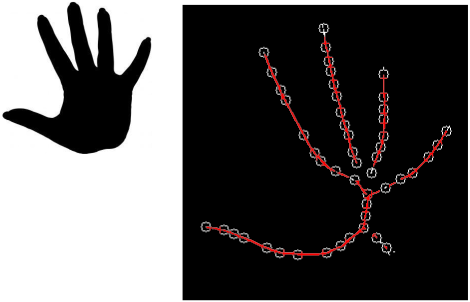
\includegraphics[width=0.4\linewidth]{./fig/features}
\caption{Ergebnis der Funktion \texttt{goodFeaturesToTrack}. Qualitätslevel: 0.1 - gewünschte Anzahl von Ecken: 50 - minimale Distanz zwischen den Ecken: 10}
\label{fig:features}
\end{figure}
Abbildung \ref{fig:features} zeigt das Ergebnis der Berechnung. Die Kreise markieren die Feature-Punkte. Wie man erkennen kann, befinden sich die Features auf der Skelettlinie. Dies ist hilfreich für die weiteren
Verbesserungen des Skeletts. Befinden sich Features außerhalb der Skelettlinien könnten die ursprüngliche Form des Skeletts und die Topologie des Objekts verfälscht werden.
\subsection{Breitensuche}
\label{subsec:breitesuche}
Der Breitensuche-Algorithmus durchsucht einen Graphen ausgehend von einem Startpunkt nach weiteren 
Knoten. Der Algorithmus sucht zunächst nur nach direkt nachfolgenden Knoten und somit in die Breite des
Graphen. Knoten, die bereits besucht wurden, werden markiert. Wurde ein Knoten noch nicht besucht, wird er
in eine \emph{Queue} (Warteschlange) aufgenommen.\\
Mittels Breitensuche sollen Pfade zwischen den markanten Punkten auf dem Skelett gefunden werden. Die markanten Punkte entsprechen Knoten in einem Graphen. Für die Nachbarschaftsbeziehung zwischen zwei
Knoten wird ein Nachbarschaftsmaß definiert. Abbildung \ref{fig:suchdistanz_naechster_nachbar} zeigt, wie überprüft wird, ob ein Punkt in einem festgelegten Intervall des Punktes $(x,y)$ liegt. Es wird eine Suchdistanz für beide Richtungen festgelegt. Sie
wird entsprechend der minimalen Distanz, die zwischen markanten Punkten erlaubt ist, gewählt (Abschnitt \ref{subsec:features}). \\
Erst wird in x-Richtung gesucht, dann in y-Richtung. Fällt der Punkt in das Intervall, wird er als besucht markiert und
mit dem Punkt $(x,y)$ verbunden. In Anhang \ref{anhang:quellcode} befindet sich der Quellcode zur Breitensuche.
%TODO: Noch weiter beschreiben: Übersicht über den Algorithmus. Bis jetzt noch ziemlich durcheinander
\begin{figure}[htbp]
\centering
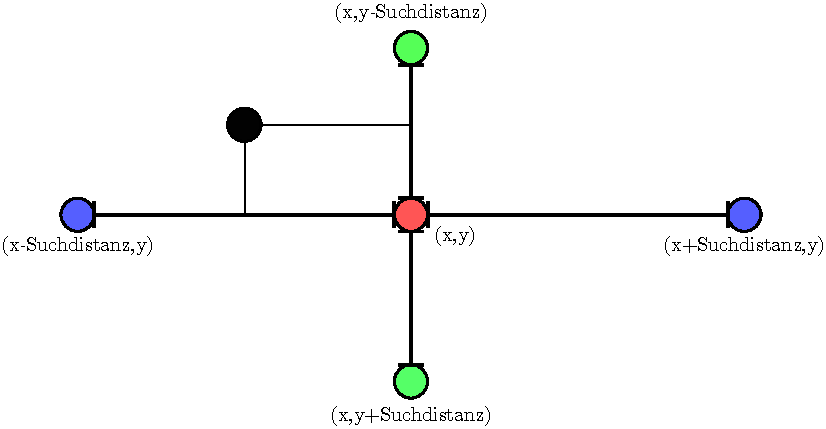
\includegraphics[width=1.0\linewidth]{./fig/suchdistanz_naechster_nachbar}
\caption{Das aufgespannte Suchkreuz vom Punkt $(x,y)$ (rot) aus. Für den schwarzen Punkt wird überprüft, ob er in den festgelegten Suchintervallen des Punktes $(x,y)$ liegt.}
\label{fig:suchdistanz_naechster_nachbar}
\end{figure}\\
Das Ergebnis des Algorithmus ist in Abbildung \ref{fig:hand_BFS} im Vergleich zum vorigen Skelett zu sehen.
Das Skelett besitzt nun zusammenhängende Komponenten. Auffällig jedoch sind die Ausläufer, die auf die 
Vorgehensweise des Breitensuchealgorithmus zurückzuführen sind. Wird die Suchdistanz zu groß gewählt,
findet der Algorithmus mehrere Nachfolger, die er dann mit dem aktuellen Punkt verbindet. Das Ergebnis
sind fächerartige Ausläufer, da der Algorithmus in die Breite sucht. %TODO Besser beschreiben...
\begin{figure}[htbp]
	\centering
	\begin{minipage}{5cm}
		\centering
		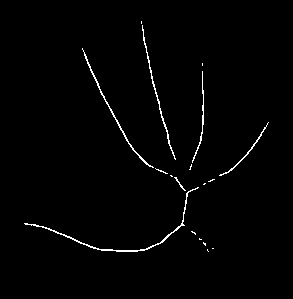
\includegraphics[width=1.0\linewidth]{./fig/hand-skelett}
	\end{minipage}
	\hspace{2cm}
	\begin{minipage}{5cm}
		\centering
		
\includegraphics[width=1.0\linewidth]{./fig/hand-bfs}
	\end{minipage}
	\caption{Ergebnis der Breitensuche. TODO Bilder schöner}
	\label{fig:hand_BFS}
	\end{figure}
\subsection{Tiefensuche}
\label{subsec:tiefensuche}
Wie bei der Breitensuche wird ausgehend von einem Startknoten ein Graph nach weiteren Knoten durchsucht. 
Im Gegensatz zur Breitensuche erfolgt das Traversieren des Graphens in die Tiefe. Wurde ein Nachfolgeknoten
gefunden, wird für diesen weiter geprüft, ob er ebenfalls einen Nachfolgeknoten besitzt. Dies wird
solange wiederholt (rekursiv) bis kein Nachfolgeknoten mehr gefunden werden kann. Mittels \emph{Backtracking} wird der Pfad zurückverfolgt. Anschließend wird ein neuer Knoten als Startpunkte gesucht, der noch nicht besucht wurde und das Durchsuchen nach nächsten Nachbarn wird für diesen Knoten wiederholt.\\
Die Suche nach dem nächsten Nachbarn funktioniert wie bei der Breitensuche (Abbildung \ref{fig:suchdistanz_naechster_nachbar}). Der Quellcode zum Algorithmus befindet sich im Anhang \ref{anhang:quellcode}. \\
Das Ergebnis ist in Abbildung \ref{fig:hand_DFS} zu sehen. Es fällt auf, dass es noch Lücken im Skelett gibt, was auf die Suchdistanz zurückzuführen ist. Ist sie zu klein, können keine weiteren Punkte im Umkreis des aktuellen Punktes gefunden werden und der Algorithmus endet für diesen Pfad. 
\begin{figure}[htbp]
	\centering
	\begin{minipage}{5cm}
		\centering
		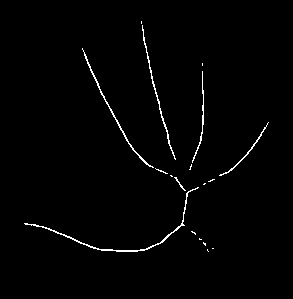
\includegraphics[width=1.0\linewidth]{./fig/hand-skelett}
	\end{minipage}
	\hspace{2cm}
	\begin{minipage}{5cm}
		\centering
		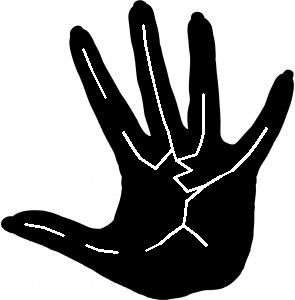
\includegraphics[width=1.0\linewidth]{./fig/hand-dfs}
	\end{minipage}
	\caption{Ergebnis der Tiefensuche.}
	\label{fig:hand_DFS}
	\end{figure}\\
Das Skelett, welches aus der Tiefensuche entsteht, bedarf demnach einer Nachbearbeitung. Die Idee ist, Punkte zu finden, die keinen Nachfolger besitzen und für diese Punkte den nächsten Nachbarn zu bestimmen. Dies wird mittels eines Ansatzes realisiert, der zwischen allen Punkten ohne Nachfolger den euklidischen Abstand bestimmt und den Punkt als nächsten Nachbar wählt, der den minimalen Abstand zu dem fest gewählten Punkt hat. In Abbildung \ref{fig:hand-punkte-ohne-nachfolger} wurden die Punkte ohne Nachfolger eingezeichnet. Diese befinden sich
genau am Ende eines Pfades. Sie entsprechen den Blättern des Baumes, der bei der Tiefensuche für einen Startknoten entsteht. 
\begin{figure}[htbp]
\centering
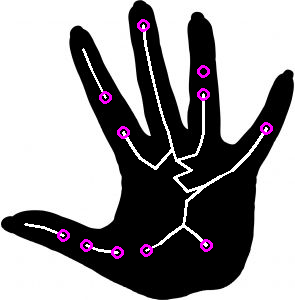
\includegraphics[width=0.4\linewidth]{./fig/hand-DFS-ohne-nachfolger}
\caption{Punkte ohne Nachfolger nachdem das Skelett nachgezeichnet wurde (markiert mit Kreisen).}
\label{fig:hand-punkte-ohne-nachfolger}
\end{figure}
Diese Punkte wurden nun miteinander verbunden. Wie in Abbildung \ref{fig:hand-DFS-endergebnis} zu sehen ist,
wurden die Punkte ohne Nachfolger, die am nächsten beieinander sind, miteinander verbunden (rote Linien). Obwohl zwei Punkte falsche Verbindungen erzeugen, liefert der Algorithmus ein gutes Ergebnis für das Skelett. Durch Einführung weiterer Bedingungen - beispielweise, ob ein Punkt bereits verbunden ist - könnten auch diese Ausläufer eliminiert werden. 
\begin{figure}[htbp]
\centering
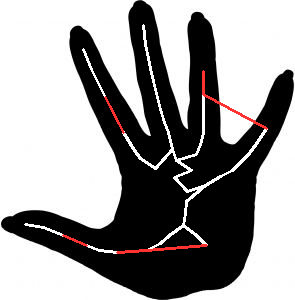
\includegraphics[width=0.4\linewidth]{./fig/hand-DFS-endergebnis}
\caption{Ergebnis der Tiefensuche}
\label{fig:hand-DFS-endergebnis}
\end{figure}
\subsection{Diskussion}
Beide Algorithmen liefern zufriedenstellende Ergebnisse bei der Verbesserung der Skelettqualität. In beiden
Fällen besteht Pixelkonnektivität und somit ein Zusammenhang zwischen den Skelettkomponenten. Die Ergebnisse
der beiden Algorithmen sind jeweils unterschiedlich aufgrund ihrer Vorgehensweise bei der Traversierung der Punkte. Die Skelette der beiden Algorithmen die geometrischen Eigenschaften des ursprünglichen Objektes gut wieder. Bei der Breitensuche sowie der Tiefensuche werden die Finger der Hand
nachgezeichnet. Nur im Bereich des Handballen entstehen - besonders bei der Breitensuche - Ausläufer im Skelett. Abhängig von der Anwendung muss man entscheiden, ob diese Ausläufer stören könnten.\\
Ein weiterer Faktor, der die Form des modifizierten Skeletts besonders beeinflusst, ist die Suchdistanz zum
Finden der nächsten Nachbarn. Wird sie zu groß gewählt, werden viele Nachbarn gefunden und somit auch
mehrere Wege von einem Punkt aus (Beispiel Breitensuche). Ist sie zu klein, entstehen Lücken im Skelett
und die Konnektivität zwischen den Skelettlinien ist nicht mehr gegeben. Man muss für jedes Bild beziehungsweise für jedes Bildobjekt entscheiden, welche Suchdistanz sich am besten eignet. Dies kann
bei der Anwendung der beiden Algorithmen auf den Videostream der Kinect hinderlich sein, da die Suchdistanz von Bild zu Bild unterschiedlich sein kann.  